\documentclass[journal]{IEEEtran}
\usepackage[a5paper, margin=10mm, onecolumn]{geometry}
\usepackage{amsmath,amssymb,amsfonts,amsthm}
\usepackage{mathtools}
\usepackage{gvv-book}
\usepackage{gvv}
\usepackage{hyperref}

\begin{document}

\title{5.2.48}
\author{Puni Aditya - EE25BTECH11046}
\maketitle

\textbf{Question:}

Solve the following system of linear equations.
\begin{align*}
    x+y+z&=1 \\
    2x+3y+2z&=2 \\
    ax+ay+2az&=4
\end{align*}

\textbf{Solution:}

\begin{align*}
    \myvec{1 & 1 & 1 \\ 2 & 3 & 2 \\ a & a & 2a}\myvec{x\\y\\z} &= \myvec{1\\2\\4}
\end{align*}
\begin{align}
    \myaugvec{3}{
        1 & 1 & 1 & 1 \\
        2 & 3 & 2 & 2 \\
        a & a & 2a & 4
    }
    \xleftrightarrow{\text{R}_3 \to \frac{1}{a}\text{R}_3, a \neq 0}
    \myaugvec{3}{
        1 & 1 & 1 & 1 \\
        2 & 3 & 2 & 2 \\
        1 & 1 & 2 & \frac{4}{a}
    }
\end{align}
\begin{align}
    \xleftrightarrow[\text{R}_3 \to \text{R}_3 - \text{R}_1]{\text{R}_2 \to \text{R}_2 - 2\text{R}_1}
    \myaugvec{3}{
        1 & 1 & 1 & 1 \\
        0 & 1 & 0 & 0 \\
        0 & 0 & 1 & \frac{4}{a} - 1
    }
    \xleftrightarrow{\text{R}_1 \to \text{R}_1 - \text{R}_2}
    \myaugvec{3}{
        1 & 0 & 1 & 1 \\
        0 & 1 & 0 & 0 \\
        0 & 0 & 1 & \frac{4}{a} - 1
    }
\end{align}
\begin{align}
    \xleftrightarrow{\text{R}_1 \to \text{R}_1 - \text{R}_3}
    \myaugvec{3}{
        1 & 0 & 0 & 2 - \frac{4}{a} \\
        0 & 1 & 0 & 0 \\
        0 & 0 & 1 & \frac{4}{a} - 1
    }
\end{align}
\begin{align}
    \myvec{x\\y\\z} &= \myvec{2 - \frac{4}{a} \\ 0 \\ \frac{4}{a} - 1},\text{ }a \neq 0 \label{eq:65}
\end{align}
For $a=0$, the third equation becomes $0=4$, which is inconsistent. Therefore, no solution exists for $a=0$. \\ \\
\textbf{Example:} \\
Let
\begin{align*}
    a = 2
\end{align*}
\begin{align*}
    x+y+z&=1 \\
    2x+3y+2z&=2 \\
    2x+2y+4z&=4
\end{align*}
\begin{align*}
    \myvec{1 & 1 & 1 \\ 2 & 3 & 2 \\ 2 & 2 & 4}\myvec{x\\y\\z} &= \myvec{1\\2\\4}
\end{align*}
Using \eqref{eq:65},
\begin{align}
    \myvec{x\\y\\z} &= \myvec{0 \\ 0 \\ 1}
\end{align}

\begin{figure}[h!]
    \centering
    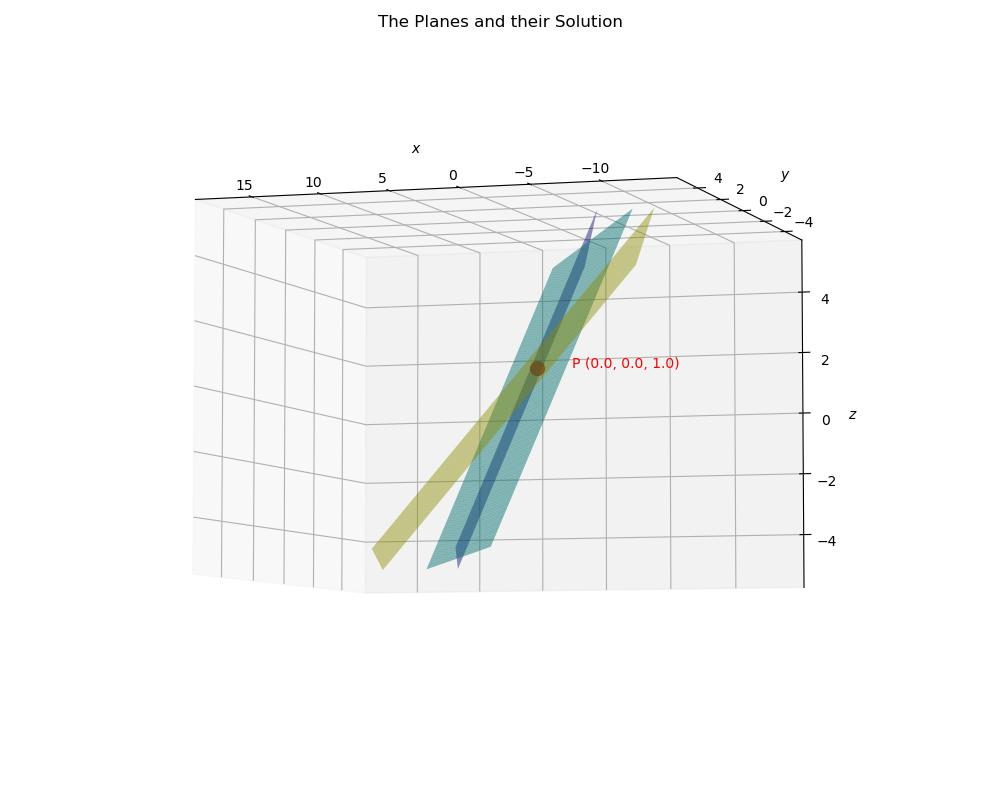
\includegraphics[width=\columnwidth]{figs/plot_c.jpg}
    \caption*{Plot}
    \label{fig:fig}
\end{figure}

\end{document}
